\documentclass{standalone}
\usepackage{tikz}
\usepackage{tabularray}
\usepackage{hyperref}
\usepackage{fontawesome7}
\usetikzlibrary{shapes.geometric, arrows, calc}
\tikzstyle{block} = [rectangle, rounded corners,
minimum width=3cm,
minimum height=1cm,
align=center,
draw]

\begin{document}

    \begin{tikzpicture}[scale=1, transform shape, gray]
      \begin{scope}[local bounding box = internals]
        \def\outcoord{9.5}
        \def\incoord{-4}

        \node (energy_out) [block, minimum height = 4cm] at (0,0) {Energy output \\ \footnotesize PVlib};
        \node[anchor= south east, text =blue] at (energy_out.south east) {\footnotesize \href{https://github.com/SjdTl/Magrivoltaics/blob/main/modules/energyOutput.py}{energyOutput.py}};
        \node (energy_used) [block, minimum height = 2cm, anchor=north, yshift=-0.25cm] at (energy_out.south) {Energy usage};
        \node[anchor= south east, text =blue] at (energy_used.south east) {\footnotesize \href{https://github.com/SjdTl/Magrivoltaics/blob/main/modules/energyUsage.py}{energyUsage.py}};
        \node (subtract) [circle, draw, yshift=-0.5cm, xshift=1cm, inner sep = 0pt, minimum size = 0.5cm] at (energy_out.south east) {\Large\textbf{$-$}};
        
        % ENERGY INPUTS
        \def\x{11}%
          \path (energy_out.north west)--(energy_out.south west) foreach \j in {1,...,\x} {%
          coordinate [pos=1/(\x + 1)*\j] (y\j)};%
          \foreach \i/\name  in {1/latitude, 2/longitude, 3/elevation, 4/height, 5/azimuth, 6/tilt, 7/rated power, 8/area, 9/panel area, 10/row width, 11/pitch}  %
            \draw[<-] (y\i) -- (y\i -| \incoord,0) node[anchor=east] (x\i){\name};%
          
        
        \draw[->] ($(energy_out.east)+(0,-0.5)$)  node[anchor=south west] {energy out} -| (subtract.north) node[pos=0.4] {\slash};
        \draw[->] (energy_used.east)  node[anchor=north west] {energy usage} -| (subtract.south) node[pos=0.4] {\slash};
        \draw[->] (subtract.east) -| +(3,-1.5) node[pos=0.3] {\slash} node[pos=0.3, above] {energy export} node(economic) [block, minimum height=3cm, anchor=north] {Economics};
        \node[anchor= south east, text =blue] at (economic.south east) {\footnotesize \href{https://github.com/SjdTl/Magrivoltaics/blob/main/modules/economics.py}{economics.py}};
        \draw[->] (energy_used.east -| subtract.south) -- (energy_used.east -| \outcoord, 0) node[anchor=west] {Energy usage [kWh]};
        \draw[->] (subtract.east -| economic.north) -- (subtract.east -| \outcoord, 0) node[anchor=west] {Energy export [kWh]};
        \draw[->] ($(energy_out.east -| subtract.north)+(0,-0.5)$) -- ($(energy_out.east -| \outcoord, 0)+(0,-0.5)$) node[anchor=west] {Energy output [kWh]};
        \draw[->] ($(energy_out.east)+(0,0.5)$)  node[anchor=south west] {irradiation} -| ($(energy_out.north -| economic.north)+(0,-0.5)$) node[pos=0.3] {\slash} node(agriculture) [anchor=south, block, minimum height=3cm] {Agriculture};
        \draw[->] ($(energy_out.east -| agriculture.south)+(0,0.5)$) -- ($(energy_out.east -| \outcoord,0)+(0,0.5)$) node[anchor=west] {Irradiation [kWh/m$^2$]};
        \node[anchor= south east, text =blue] at (agriculture.south east) {\footnotesize \href{https://github.com/SjdTl/Magrivoltaics/blob/main/modules/agriculture.py}{agriculture.py}};
        
        \def\x{5}%
          \path (economic.north west)--(economic.south west) foreach \j in {1,...,\x} {%
          coordinate [pos=1/(\x + 1)*\j] (y\j)};%

        \draw[->] ($(y8)+(-0.33,0)$) |- (y1);
        \draw[->] ($(y9)+(-0.66,0)$) |- (y2);
        \draw[->] ($(y10)+(-1.166,0)$) -- +(0,-2) node (divide) [anchor=north, circle, draw, minimum size = 0.5cm, inner sep=0pt] {\large \textbf{$/$}};  
        \draw[->] ($(y11)+(-1.66,0)$) |- (divide.west);
        \draw[->] (divide.south) |- (y3);

        \draw[<-] (y4) -- (y4 -| \incoord,0) node[anchor=east] {subsidy}; 
        \draw[<-] (y5) -- (y5 -| \incoord,0) node[anchor=east] {lifetime}; 
        % % ECONOMIC INPUTS
        % \def\x{2}%
        %   \path (economic.north west)--(economic.south west) foreach \j in {1,...,\x} {%
        %   coordinate [pos=1/(\x + 1)*\j] (y\j)};%
        %   \foreach \i/\name  in {1/subsidy, 2/lifetime}  %
        %     \draw[<-] (y\i) -- (y\i -| \incoord,0) node[anchor=east] (x\i){\name};%

        % ECONOMIC OUTPUTS
        \def\x{4}%
        \path (economic.north east)--(economic.south east) foreach \j in {1,...,\x} {%
        coordinate [pos=1/(\x + 1)*\j] (y\j)};%
        \foreach \i/\name/\bus  in {1/LCOE [eur\slash MWh]/, 2/ROI/, 3/Maintenance cost [eur\slash y]/, 4/Energy price [eur\slash kWh]/}  %
        \draw[->] (y\i) -- (y\i -| \outcoord, 0) node[anchor=west] (x\i){\name} node[midway] {\bus};%
        

        % AGRICULTURAL INPUTS
        \def\x{1}%
        \path (agriculture.north west)--(agriculture.south west) foreach \j in {1,...,\x} {%
        coordinate [pos=1/(\x + 1)*\j] (y\j)};%
        \foreach \i/\name  in {1/crop type}  %
        \draw[<-] (y\i) -- (y\i -| \incoord,0) node[anchor=east] (x\i){\name};%
        % AGRICULTURAL OUTPUTS
        \def\x{1}%
        \path (agriculture.north east)--(agriculture.south east) foreach \j in {1,...,\x} {%
        coordinate [pos=1/(\x + 1)*\j] (y\j)};%
        \foreach \i/\name/\bus  in {1/Crop impact [kW\slash m$^2$]/\slash}  %
        \draw[->] (y\i) -- (y\i -| \outcoord, 0) node[anchor=west] (x\i){\name} node[midway] {\bus};%
          
      \end{scope}
      \draw[draw] ($(internals.north west)+(2.5,0.25)$) rectangle ($(internals.south east)+(-4.5,-0.25)$);

      \coordinate (corner) at ($(internals.south west) + (2.5,-0.25)$);
      \coordinate (rightcorner) at ($(internals.south east) + (-7,-0.25)$);
      \node[anchor=south west, above right] at (corner) {\Large Interface \faPython};

      \begin{scope}[shift= {($(corner)+(0,-0.5)$)}]
          \draw[->] (0,0) -- +(1,0) node[midway] {\slash} node[anchor=west] {= monthly variable for the average year};  
          \draw[->] (0,-0.5) -- +(1,0) node[anchor=west] {= one time variable for the lifetime};  
      \end{scope}
      \begin{scope}[shift= {($(rightcorner)+(0,-0.5)$)}]
        \node[align=left] at (0,0) {\footnotesize In general, most variables are fixed: \\ \footnotesize only one changes};
      \end{scope}
    \end{tikzpicture}

\end{document}